\chapter{Validität und Einschränkungen}
\label{chap:gueltigkeit}

Eine umfassende Berücksichtigung der Validitätseinschränkungen ist für die Bewertung der Relevanz einer empirischen Studie von großer Bedeutung.
Jede Arbeit hat durch die verwendete Methodik Einschränkungen hinsichtlich ihrer Validität \cite{campbell2015experimental}.
Auch diese Arbeit hat gewisse Limitationen, die in diesem Kapitel erörtert werden.
\Citet{Runeson2009} stellen eine mögliche Klassifizierung der verschiedenen Faktoren vor, die Einfluss auf die Validität haben.
Dieses Kapitel ist entsprechend die vier Klassen \emph{konstruktionsbedingte Validität}, \emph{Interne Validität}, \emph{Reliabilität} und \emph{Externe Validität} strukturiert.

\section{Konstruktionsbedingte Validität}

Dieser Aspekt der Validität (original \emph{Construct validity}) drückt aus, inwieweit die verwendete Methodik tatsächlich die gestellte Forschungsfrage untersucht und ein Ergebnis liefert, das diese Forschungsfrage beantwortet \cite{Runeson2009}.

Die übergeordnete Methodik der gesamten Fallstudie besteht in erster Linie aus der Anwendung des \gls{mmf} auf \jf und der anschließenden Auswertung der Ergebnisse dessen.
Der erste Schritt (die Anwendung des \gls{mmf}) wird in der Forschungsfrage erwähnt und zielt direkt auf deren Beantwortung ab.
Im zweiten Schritt (der Evaluation der Ergebnisse der Anwendung) hängt die konstruktionsbedingte Validität von den verwendeten Methoden ab.

Die Frage in den Experteninterviews wurden so konzipiert, dass sie sehr gezielte Fragen mit starkem Bezug zu den Unterfragen der \ff enthalten.
Für die erste Teilfrage wurden in einem dedizierten Teil (mit Bezug zur Granularität) Fragen zu Migrationsverfahren und deren Anwendung auf \jf gestellt.
Für die zweite Unterfrage wurden in einem weiteren Teil Fragen zur Eignung der vom \gls{arh} vorgeschlagenen \bpp für \jf gestellt.
Auch hier bezieht sich eine Frage speziell auf den in der \ff genannten Qualitätsaspekt.
Obwohl viele Fragen einen direkten Bezug zur \ff haben, kann die konstruktionsbedingte Validität trotzdem eingeschränkt sein, falls Teilnehmer die Fragen anders verstanden haben.

Die Auswertung der Feldnotizen ist dagegen nur in indirekterer Form auf die \ff ausgerichtet.
Aus den Feldnotizen geht nicht direkt hervor, ob und wie gut die \gls{arh} für das Refactoring von \jf geeignet ist.
Vielmehr geben sie einen Einblick in die Durchführung des Prozesses und die damit verbundenen Probleme, Emotionen und Anmerkungen.
Diese Stellung der Methodik ist bei der Betrachtung der Ergebnisse zu berücksichtigen.

\section{Interne Validität}

Die interne Validität ist gegeben, wenn die untersuchten Kausalbeziehungen isoliert sind und andere Kausalitäten, die das Ergebnis ebenfalls beeinflussen, bekannt sind und berücksichtigt werden \cite{Runeson2009}.

In \cref{fig:limitations} wurde versucht, mögliche Auswirkungen von erwünschten Messfaktoren auf die Schritte in dieser Arbeit sowie von unerwünschten Störfaktoren auf diese zu skizzieren.
Als Hauptstörfaktoren werden die \emph{beteiligten Personen} sowie die \emph{verwendete Methodik und Vorgehensweise} vermutet.
Dies sind jeweils nur Oberbegriffe für Sammlungen von möglichen Einflüssen.

\emph{Beteiligte Personen} bezieht sich primär darauf, welche Personen beteiligt waren.
Es sollte aber auch beinhalten, welche Probleme diese Personen mitbringen (Emotionen, Differenzen, Machtunterschiede).
Es können auch der Grad der Erfahrung der Personen, menschliches Versagen und viele andere Einflüsse beinhaltet sein, die von den beteiligten Personen ausgehen.

Der Begriff \emph{Verwendete Methodik und Vorgehensweise} bezieht sich auf den gewählten Ansatz zur Durchführung der Maßnahme.
Im Falle der Wahl der \glspl{qa} ist dies die in \cref{sec:methodik-architekturreview} beschriebene Methodik des Architekturreviews.
In den anderen Schritten bezieht es sich auf weniger formale Vorgehensweisen, beispielsweise auf die gemeinsame Filterwahl oder die Art und Weise, wie verschiedene Suchergebnisse aggregiert werden.
All diese Vorgehensweisen können Auswirkungen auf die Ergebnisse haben, die es zu minimieren gilt.

\begin{figure}
	\centering
	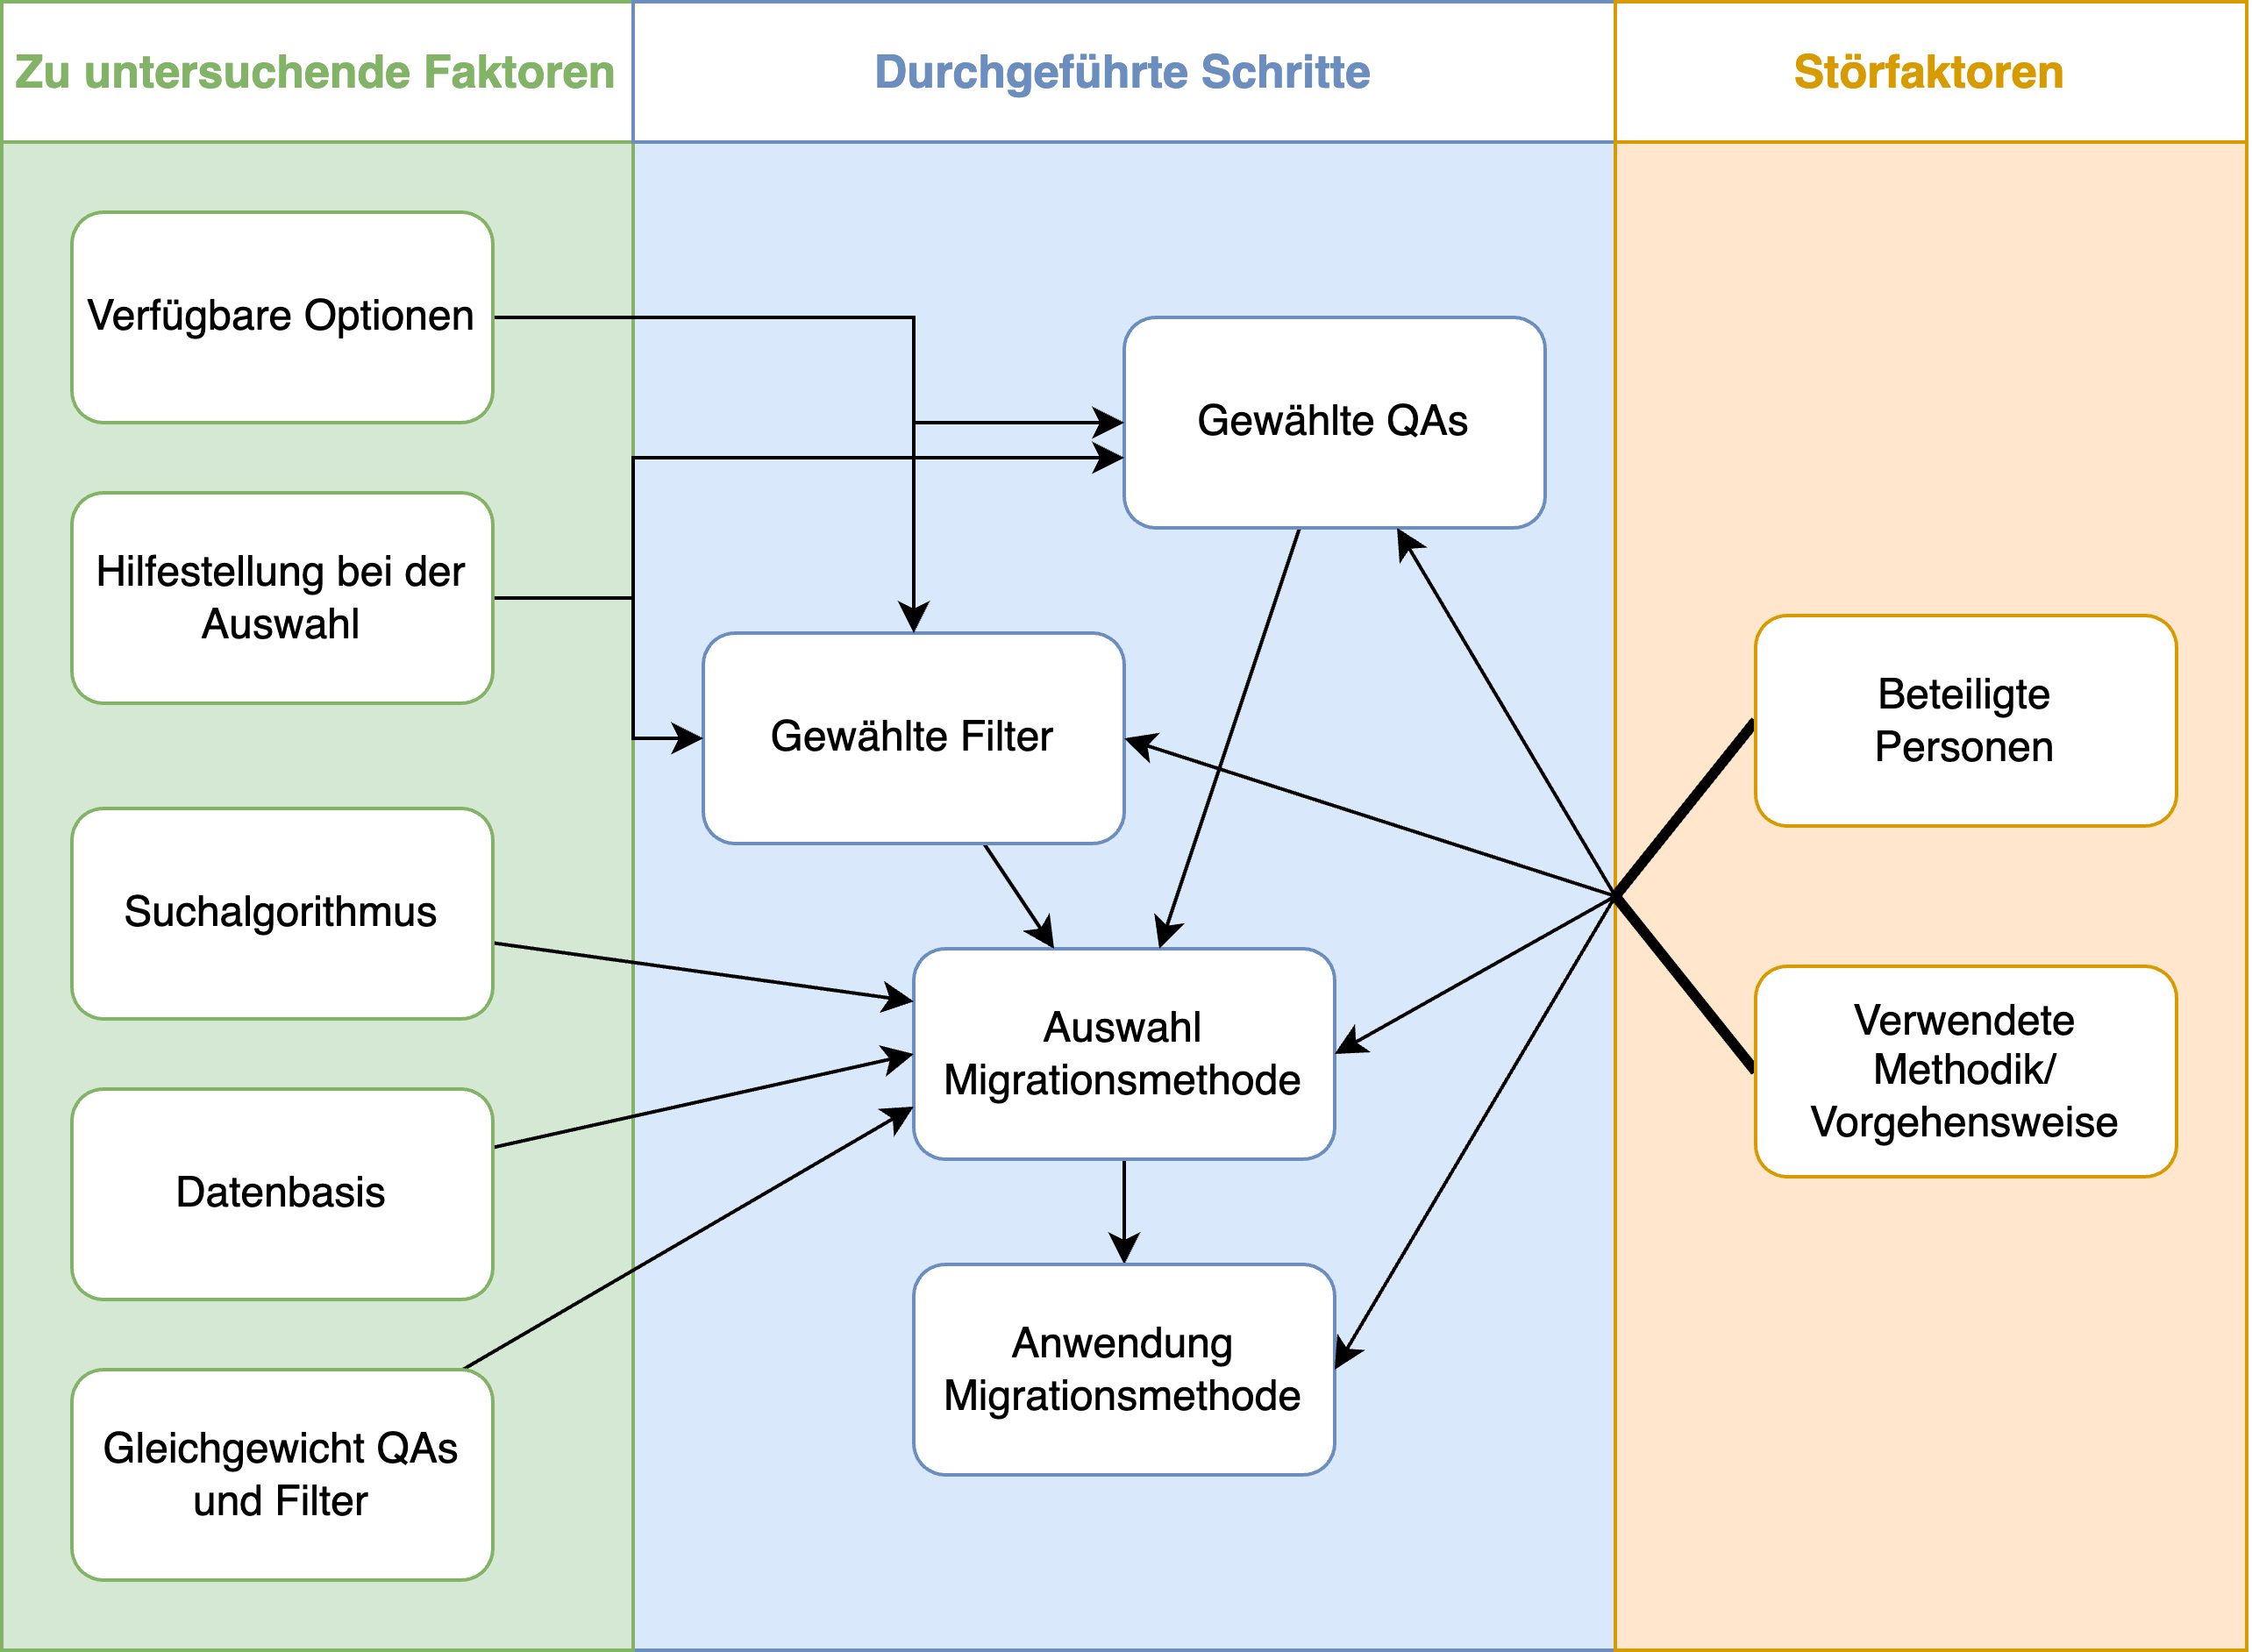
\includegraphics[width=1.0\textwidth]{limitations.drawio}
	\caption[Kausale Beziehungen der Fallstudie]{
			Kausale Beziehungen zum Ergebnis dieser Fallstudie und generell der Anwendung des \gls{arh}.
%			Einflüsse der Qualität des \gls{mmf} und \gls{arh} sowie andere Einflüsse auf das Ergebnis der Fallstudie.
		}
	\label{fig:limitations}
\end{figure}

\section{Reliabilität}

Für eine hohe Verlässlichkeit (original \emph{Reliability}) ist es wichtig, dass die Subjektivität des Autors möglichst wenig Einfluss auf die Ergebnisse der Studie hat \cite{Runeson2009}.
Im Falle dieser Arbeit ist die Reliabilität in einigen Punkten eingeschränkt.

Zum einen wurden die meisten Schritte in dieser Arbeit von nur einem Studenten durchgeführt, der nur über begrenzte Erfahrung in Software Engineering und wissenschaftlichem Arbeiten verfügt.
Dieses Risiko wurde versucht zu minimieren, indem in zumeist wöchentlichen Abständen mit dem \gls{po} von \jf und dem universitären Betreuer die durchgeführten und nächsten Schritte besprochen wurden.
Außerdem wurde das Architekturreview zur Erfassung der \glspl{qa}, die die späteren Ergebnisse maßgeblich beeinflussen, mit insgesamt fünf wichtigen Mitgliedern des Entwicklungsteams durchgeführt.
Damit sollte eine möglichst hohe Qualität der \glspl{qa} sichergestellt werden.
Insbesondere bei zu komplexen Details ist diese Strategie des Vier-Augen-Prinzips nicht möglich, da eventuell helfende Personen keine Zeit für die notwendige Einarbeitung hätten.
Konkret ist dieses Problem in der Arbeit bei der Anwendung des Migrationsverfahrens in \cref{sec:anwendung-verfahren} aufgetreten.
Hier haben ein Algorithmus und Formeln auf einer sehr tiefen Detailebene zu Problemen geführt, die vom Autor nicht in der begrenzten Zeit gelöst werden konnten.
Gleichzeitig waren sie jedoch zu komplex für andere Personen, um eventuell helfen zu können.

Die gleiche Kritik gilt für die Methodik der Feldnotizen.
Diese wurden nur von einer Person erstellt und ausgewertet, die keine Erfahrung mit dieser Methode hatte.
Die Erstellung von Feldnotizen ist unabhängig von der Unerfahrenheit mit einem gewissen Maß an Subjektivität verbunden.
Um diese Einschränkung zu minimieren, wurden für die Erhebung und Auswertung der Feldnotizen etablierte Methoden ausgewählt und vor der Anwendung umfangreiche Recherchen durchgeführt.

Eine weitere Einschränkung der Verlässlichkeit ergibt sich bei der Durchführung der Interviews.
Sowohl die Befragten als auch der Interviewer könnten an einer positiven Bewertung der Arbeit interessiert sein, wodurch gewollt oder ungewollt mehr positive Ergebnisse produziert werden könnten.
Außerdem können die persönlichen Beziehungen zu den Interviewteilnehmern und damit verbundene Sympathien und Antipathien Auswirkungen auf die Ergebnisse haben.
Um die Objektivität zu erhöhen, wurden die Befragten explizit aufgefordert, ehrliche Antworten zu geben.
Trotzdem kann eine gewisse Einschränkung nicht ausgeschlossen werden.

Darüber hinaus stellt die Auswertung der Daten generell ein Risiko für die Zuverlässigkeit dar.
Diese wurde nur von einer unerfahrenen Person durchgeführt.
Insbesondere bei der Kodierung der Daten ist eine gewisse Subjektivität unvermeidlich.
Bei der Kodierung der Feldnotizen wurde versucht, einen möglichst objektiven Kodierleitfaden zu definieren.
Die Kodierung der Experteninterviews ist naturgemäß subjektiv.
Da die Kodierung in diesem Fall aber auch nicht das Hauptergebnis ist, sondern die textliche Auswertung der Interviews wesentlich genauer beschrieben und fokussiert wird, stellt dies kein relevantes Problem dar.

\section{Externe Validität}

Die externe Validität beschreibt das Ausmaß, in dem die Ergebnisse der Studie verallgemeinert werden können \cite{Runeson2009}.
In diesem Fallbeispiel bedeutet dies konkret, inwieweit von den Ergebnissen dieser Arbeit auf mögliche andere Anwendungen der \gls{arh} geschlossen werden kann.
Externe Validität kann in der Regel nicht durch logische Maßnahmen sichergestellt werden, sondern nur durch die Annahme von Gesetzmäßigkeiten optimiert werden \cite{campbell2015experimental}.

Die externe Validität ist hoch, wenn andere Anwendungen unter ähnlichen Bedingungen statt\-fin\-den \cite{campbell2015experimental}.
Daher sind die variierenden Eingaben bei Verwendung des \gls{arh} eine wichtige Einschränkung.
Die Ergebnisse der Suche nach Migrationsverfahren und der Suche nach \bpp hängen vollständig von den gewählten \glspl{qa} und Filteroptionen ab.
Wenn andere Eingaben verwendet werden, kann dies zu einer anderen Reihenfolge der Suchergebnisse und folgend anderen Ergebnissen in der Anwendung führen.

Darüber hinaus wird die externe Validität im Bezug auf die allgemeine Anwendung des \gls{arh} durch den Spezialfall in dieser Thesis, dass die Ausgangsarchitektur eine \gls{msa} ist, weiter eingeschränkt.
Dadurch besteht eine geringere Ähnlichkeit zu anderen Anwendungsfällen mit Monolithen als Ausgangsarchitektur, was nach \Citet{campbell2015experimental} zu einer schlechteren externen Validität in diesen Fällen führt.
Auf der anderen Seite erhöht genau diese Bedingung die externe Validität in Bezug auf die Verwendung des \gls{arh} mit \glspl{msa} im Vergleich zu beispielsweise der Fallstudie von \Citet{master-marvin-knodel}.

Die einzige Maßnahme, die zur Verbesserung der externen Validität ergriffen werden kann, ist die Sicherstellung einer möglichst hohen Konstruktvalidität, internen Validität und Reliabilität, sodass zumindest die Voraussetzungen für die externe Validität optimiert sind.

%Neben der Qualität des \gls{mmf} und \gls{arh} gibt es viele andere Faktoren, die das Ergebnis im Einzelfall und auch in dieser Fallstudie beeinflussen können:
%
%\begin{itemize}
%	\item Die Auswahl der Migrationsmethode wird beeinflusst durch
%	\begin{itemize}
%		\item Qualität der \glspl{qa}
%		\item Qualität der Filter
%		\item Gleichgewicht zwischen \glspl{qa} und Filtern
%	\end{itemize}
%\end{itemize}
%
%\begin{figure}
%	\centering
%	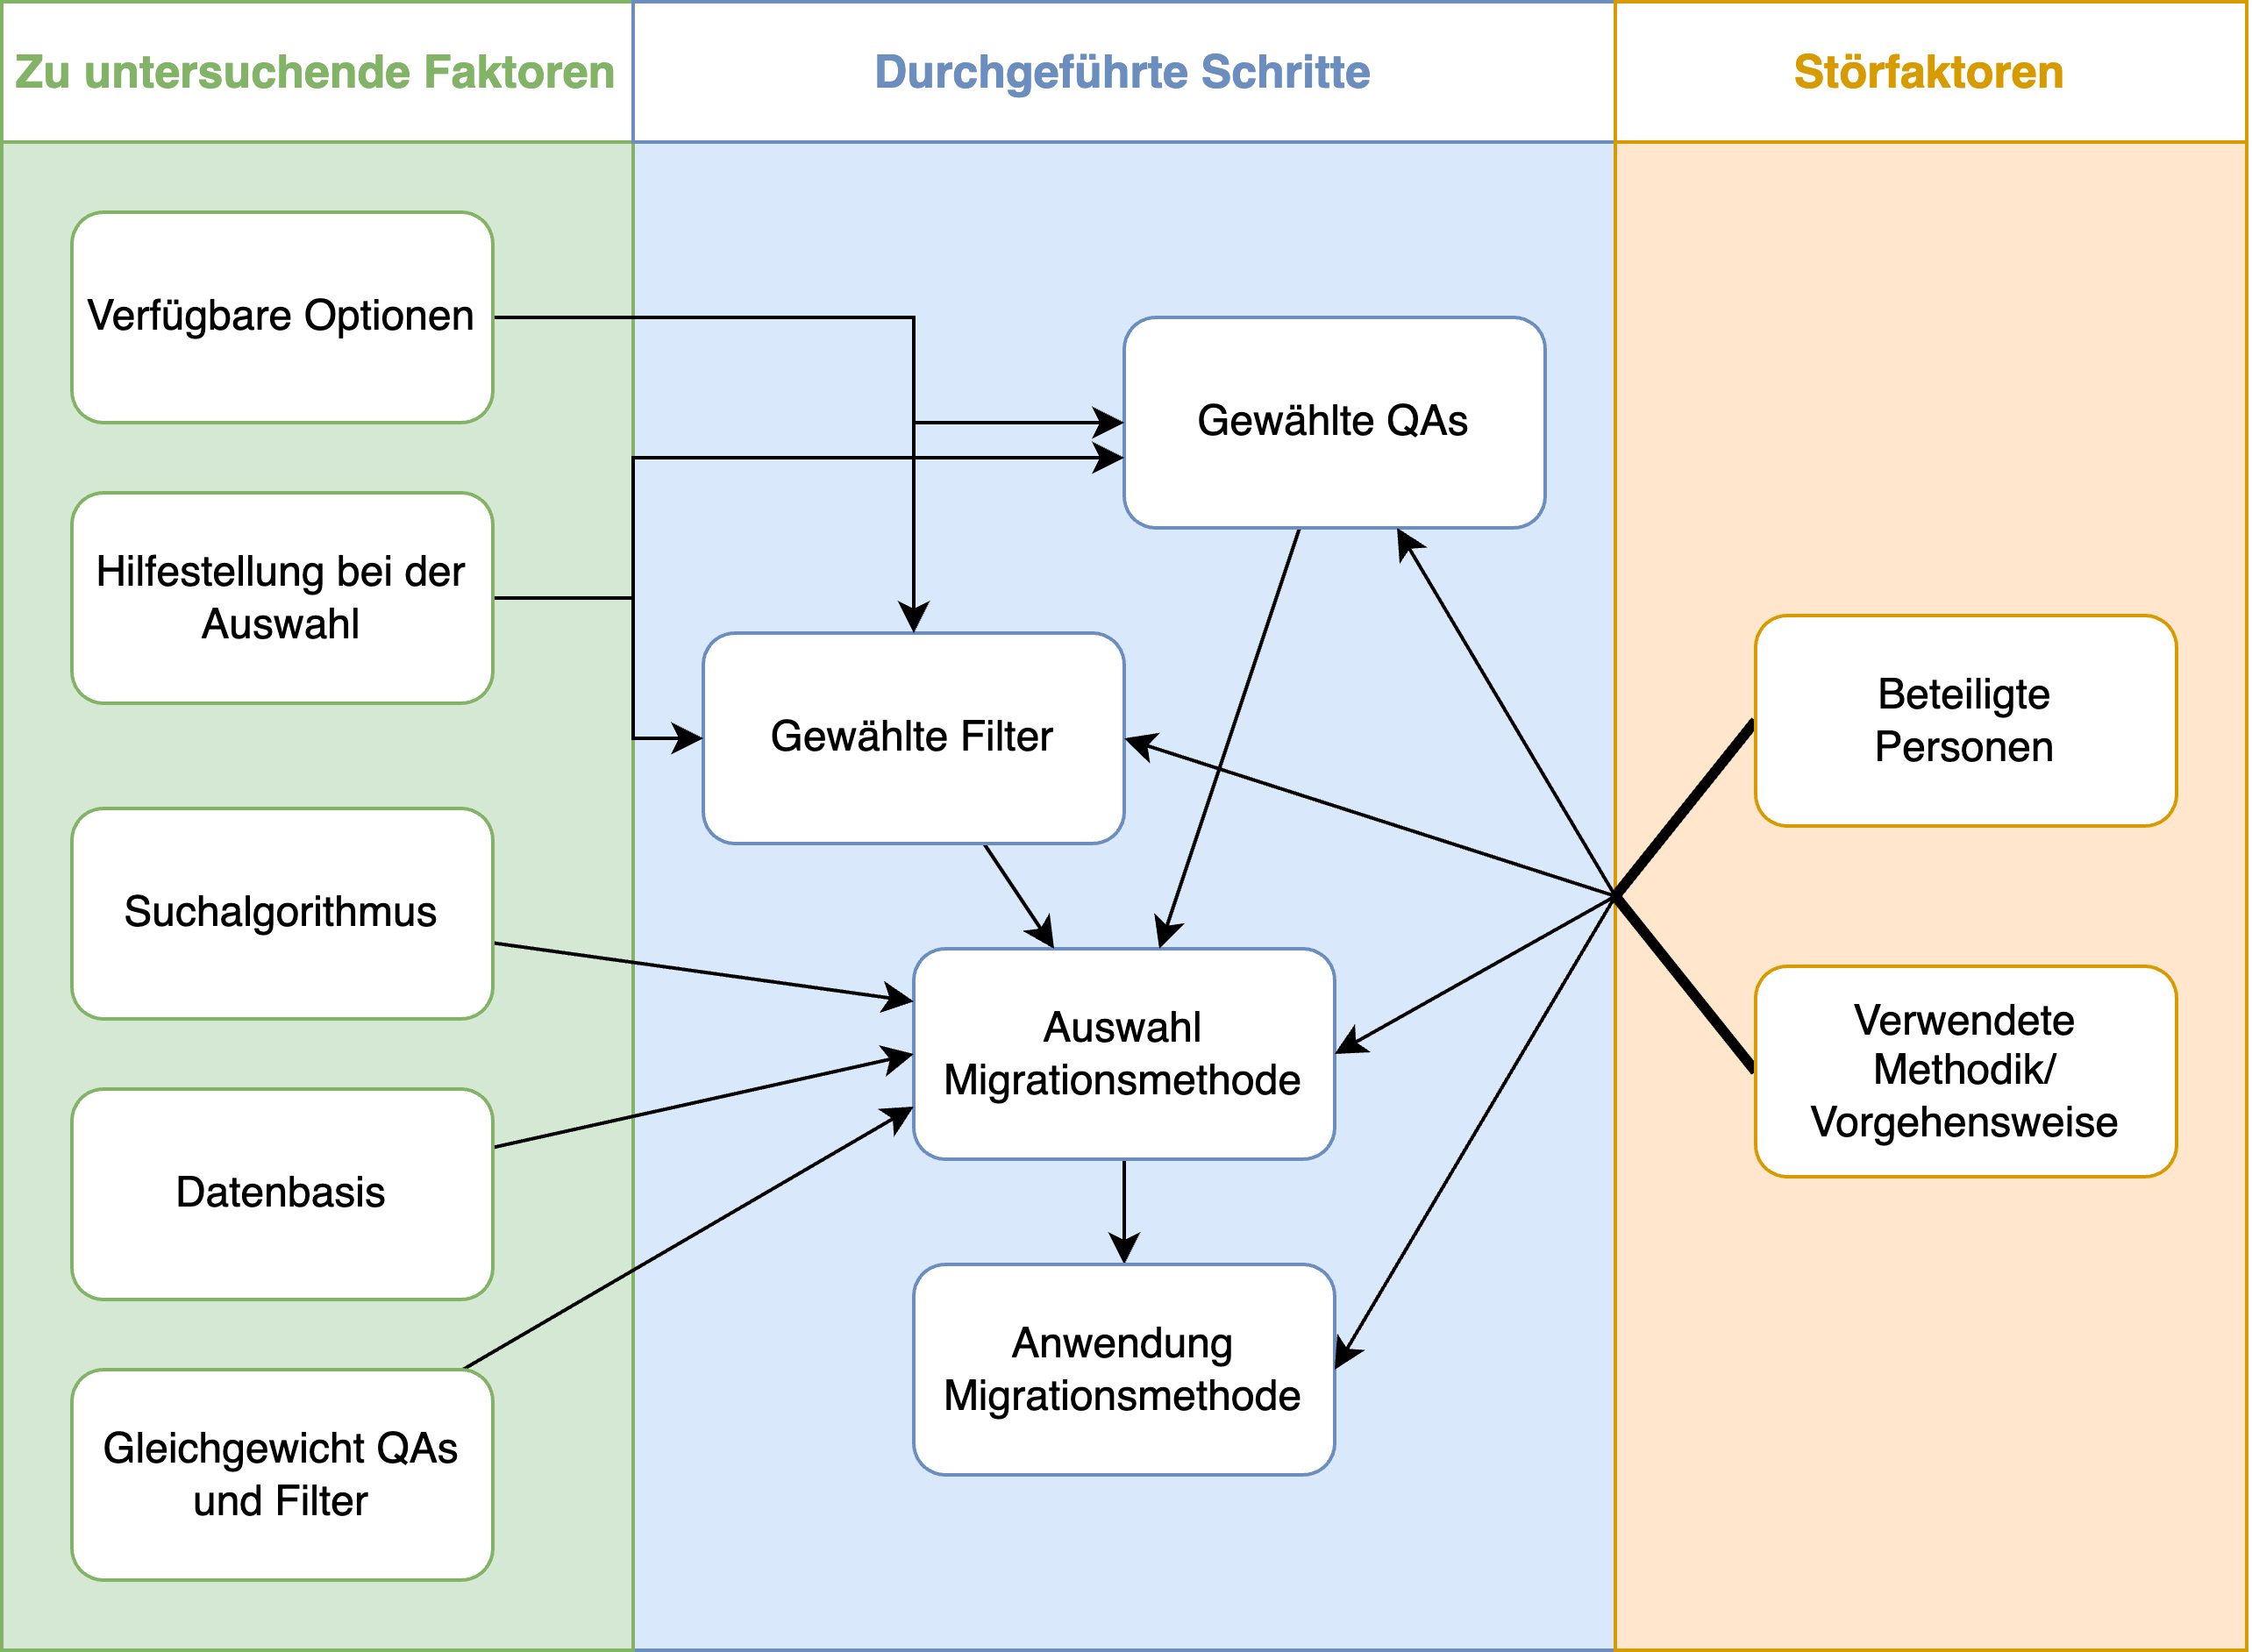
\includegraphics[width=1.0\textwidth]{limitations.drawio}
%	\caption[Einflüsse auf das Ergebnis der Fallstudie]{
%		Einflüsse der Qualität des \gls{mmf} und \gls{arh} sowie andere Einflüsse auf das Ergebnis der Fallstudie.
%	}
%	\label{fig:limitations}
%\end{figure}
%
%Phase 1:
%Das Architekturreview ist für die Migration zu einem Microservices-System von Monolithen gedacht.
%Insbesondere existiert dabei das Zielprodukt noch nicht in der Ziel Architektur.
%In unserem Fall dagegen war die Ausgangsarchitektur schon gleich der Zielarchitektur.
%Dadurch war es bei dem Architekturreview schwierig, die technische Schwierigkeit eines Szenarios einzuschätzen, da einige der Szenarios so schon umgesetzt sind und damit argumentiert werden kann, dass es dann nicht technisch schwierig ist, da es schon vorhanden ist.
%
%Nicht möglich gewesen, dass alle Stakeholder beim Architekturreview anwesend sind: Kein Kunde
%- Arbeit mit \gls{arh} wurde von unerfahrenem Softwareentwickler durchgeführt und nur für größere Schritte und Zusammenfassungen der Einzelheiten erfahrenen und wichtigeren Stakeholder konsultiert
%
%\section{Interne Validität}
%
%- hohe Komplexität bei den Experteninterviews
%- Ein Experte hat an der Thesis mitgearbeitet
%- Fragen bei den Interviews teils sehr hypothetisch
%- Interviewer ohne Erfahrung
%
%\begin{itemize}
%	\item Begrenzter Rahmen durch Bachelorarbeit
%\end{itemize}
%
